\documentclass[border=4pt]{standalone}
\usepackage{tikz}
\usetikzlibrary{arrows.meta}
\definecolor{ink}{HTML}{2A2620}
\definecolor{violet}{HTML}{5A1BA6}
\definecolor{terracotta}{HTML}{A03A2C}
\definecolor{sage}{HTML}{8AA08A}
\definecolor{inkfaint}{HTML}{7A6F62}
\begin{document}
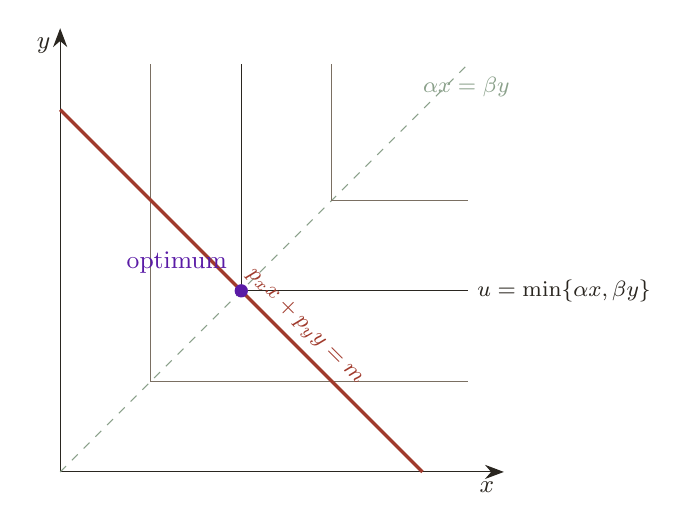
\begin{tikzpicture}[x=1.15cm,y=1.15cm,>={Stealth[length=2.4mm]},font=\small]
  \draw[->,ink] (0,0) -- (4.9,0) node[below left]{$x$};
  \draw[->,ink] (0,0) -- (0,4.9) node[below left]{$y$};
  % ray where the goods are used in proportion
  \draw[sage,dashed] (0,0) -- (4.5,4.5);
  \node[sage,right,font=\footnotesize] at (3.9,4.25) {$\alpha x=\beta y$};
  % L-shaped indifference curves
  \draw[inkfaint] (1,4.5) -- (1,1) -- (4.5,1);
  \draw[ink] (2,4.5) -- (2,2) -- (4.5,2);
  \node[ink,right,font=\footnotesize] at (4.5,2) {$u=\min\{\alpha x,\beta y\}$};
  \draw[inkfaint] (3,4.5) -- (3,3) -- (4.5,3);
  % budget line
  \draw[terracotta,very thick] (0,4) -- (4,0);
  \node[terracotta,rotate=-45,anchor=south,font=\footnotesize] at (2.55,1.45) {$p_x x+p_y y=m$};
  % optimum at the kink
  \fill[violet] (2,2) circle (2.4pt);
  \node[violet,above left,font=\small] at (1.95,2.08) {optimum};
\end{tikzpicture}
\end{document}
